\chapter{Proposed CC Mechanism in IIoT}

\section{Proposed C-LV for Congestion Control in IIoT}

In this thesis, we design congestion control scheme based on the deterministic information of population dynamics from C-LV. An IIoT has some similarities with an ecosystem. An ecosystem consists of several species that live together and interact with resources to survive and coexist. In IIoT, before forwarding data to the Internet, each sensor node has to compete to transmit their payload to the sink node through a harsh industrial environment.
IIot consists of sensor nodes that work cooperatively. Each node has a buffer, and the number of the available buffers can cause traffic flow to be initiated differently. In the C-LV model, traffic flows can be seen as species that compete for available network resources. Moreover, the number of bytes per traffic flow can be seen as the population of each traffic flow. The purpose of implementing C-LV model in IIot is designing a scheme to guarantee the coexistence of the flows as an ecosystem tries to make sure each species coexists. 

The proposed scheme provides rate adaptation by regulating the traffic flow rate at each sensor node. Therefore, each sensor node controls the rate of its traffic flow. Owing to the decentralized nature of the proposed scheme, it needs low communication overhead.




As shown in Fig. \ref{fig:letter}, each sensor node sends a packet to the sink node. Each node acts as a competing species, and the buffer capacity of the sink node can be seen as the carrying capacity of every species. Therefore, each traffic flow has the same carrying capacity in this model, i.e., 
\begin{equation}
\label{assume1}
\forall i \in \{1,2,3,...,n\},~K_i=K.
\end{equation}

\begin{figure}
	\centering
	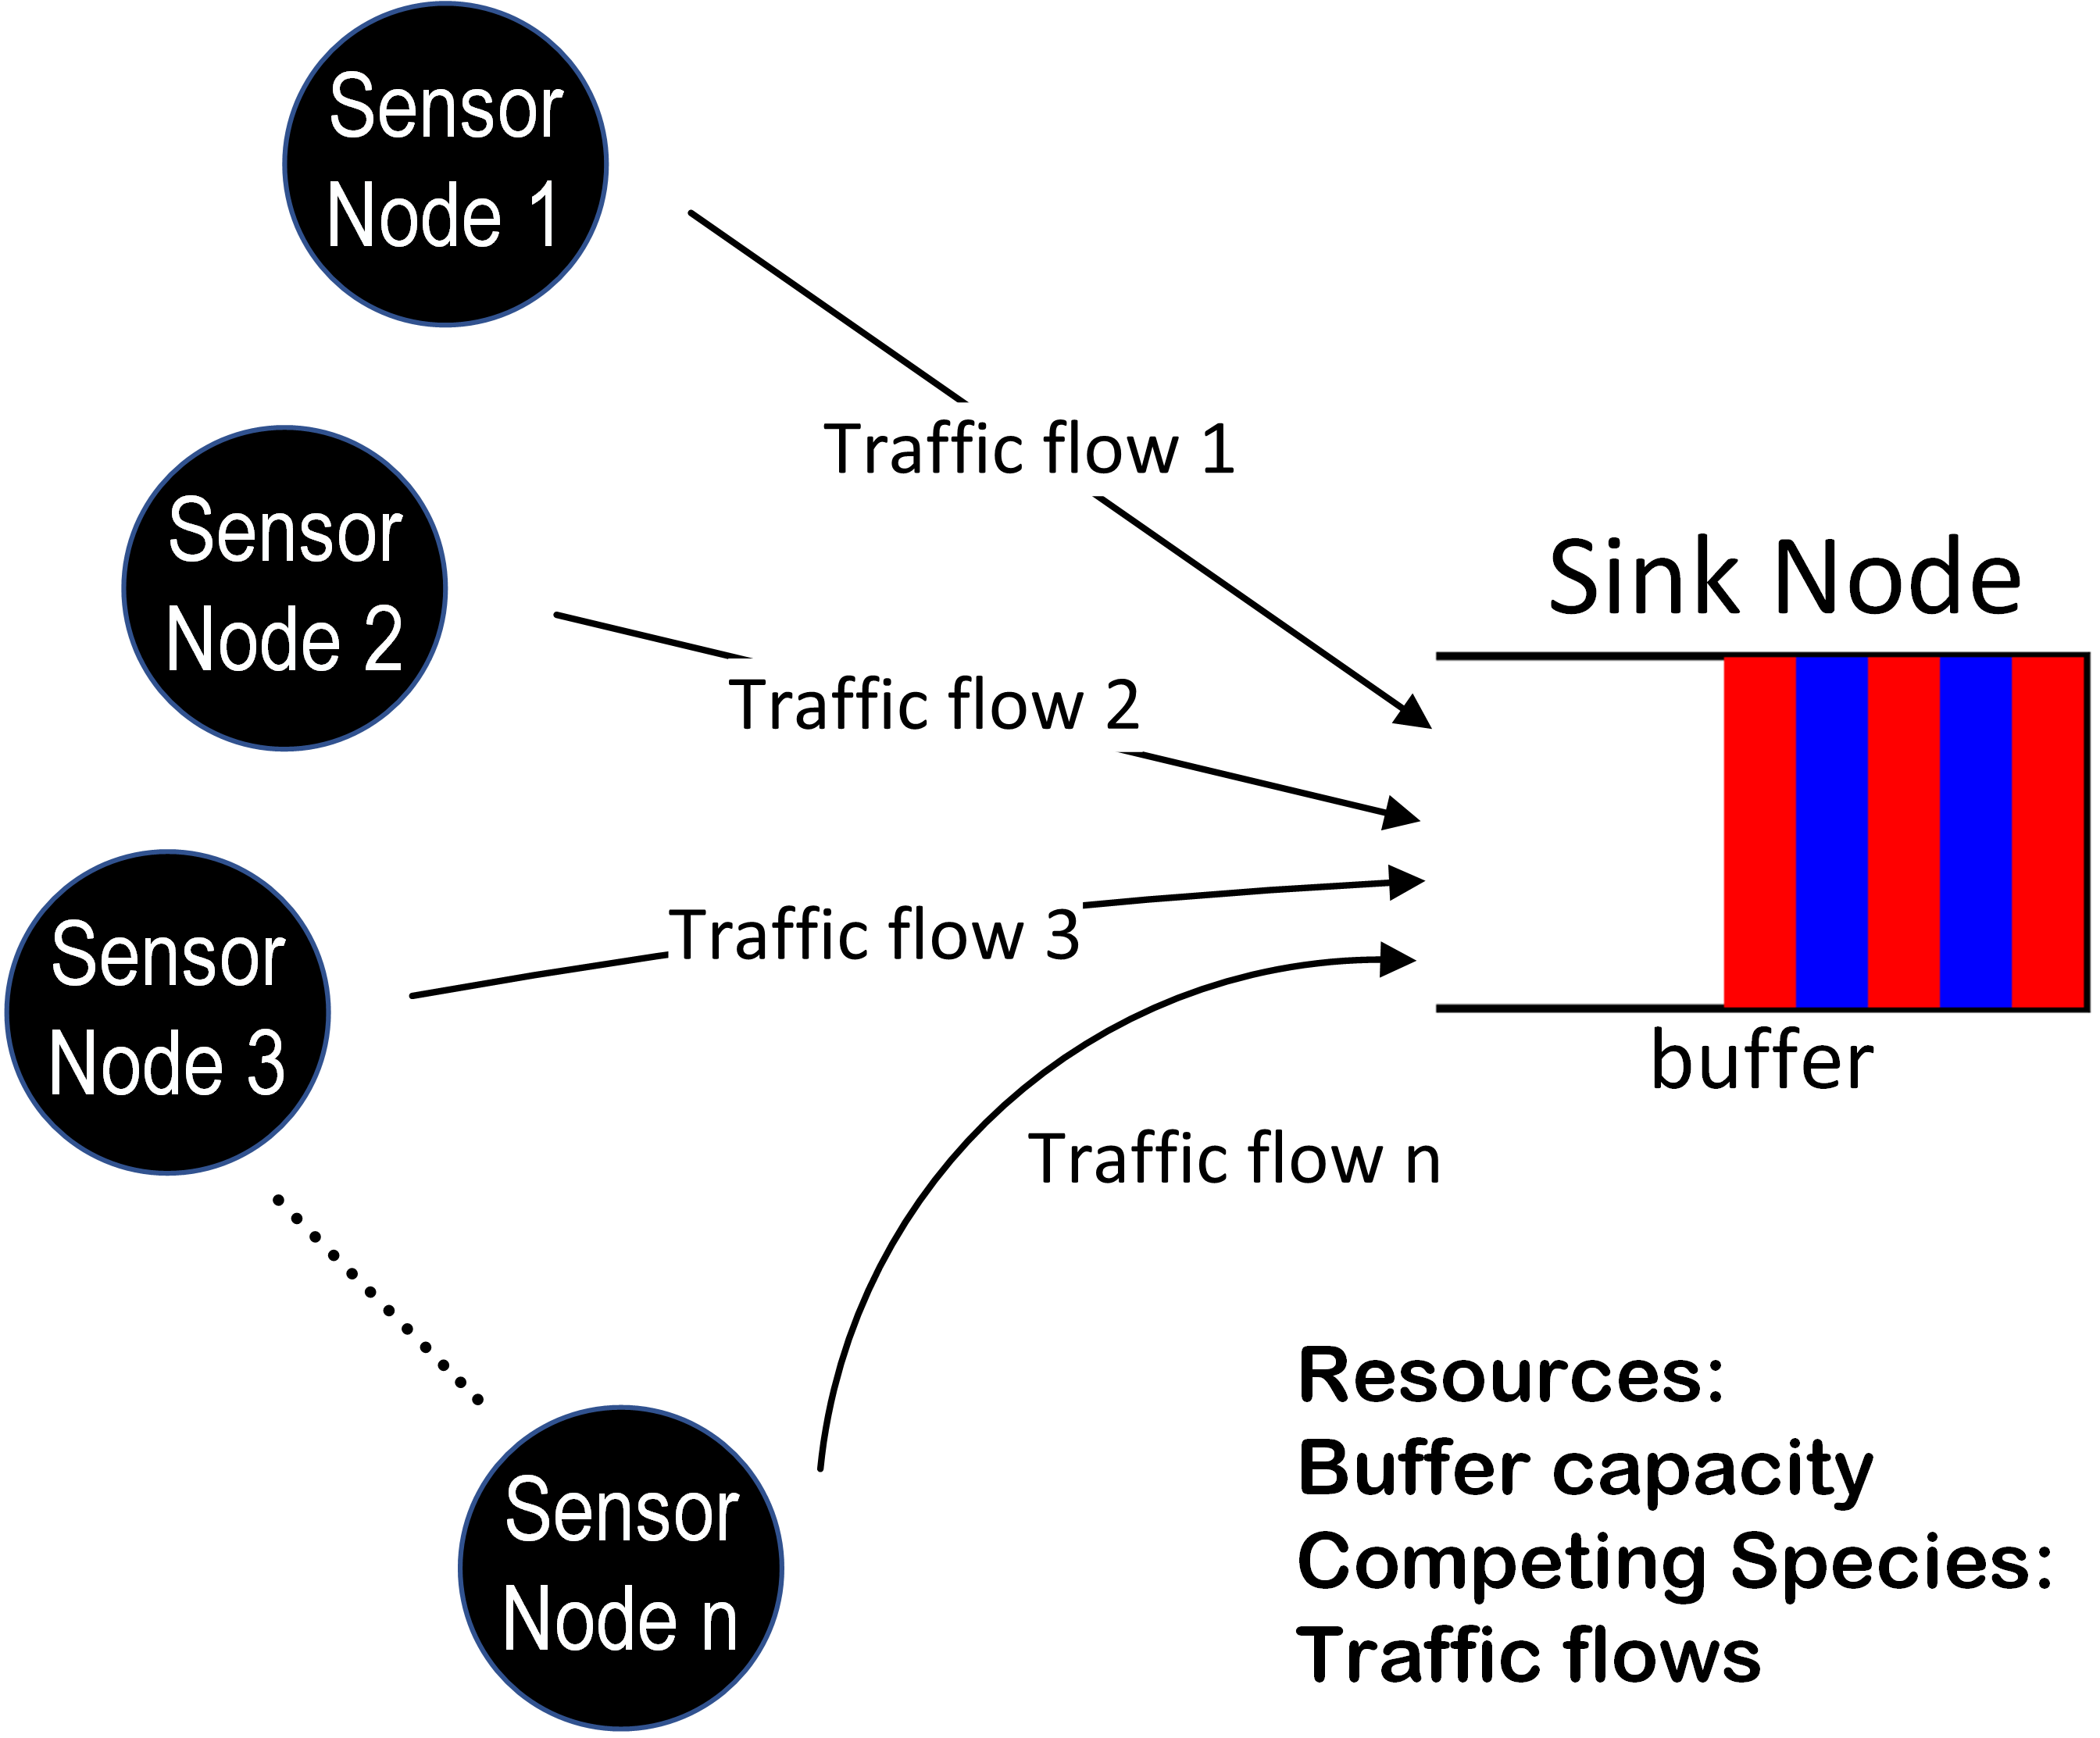
\includegraphics[width=1\linewidth]{pics/letter.png}
	\caption{Traffic flows competition in WSNs}
	\label{fig:letter}
\end{figure}



In this scheme, for simplicity, it is assumed that 

\begin{equation}
\label{assume2}
\forall i,j \in \{1,2,3,...,n\},~\alpha_{ij}=\alpha,~\text{when}~i \neq j,
\end{equation}

\begin{equation}
\label{assume3}
\forall i \in \{1,2,3,...,n\},~\alpha_{ii}=\beta,
\end{equation}
and

\begin{equation}
\label{assume4}
\forall i \in \{1,2,3,...,n\},~r_{i}=r.
\end{equation}




Therefore, the transmission rate of each traffic flow is determined periodically by,

\begin{equation}
\label{jaran}
\frac{dx_i}{dt}=rx_i(1-\frac{\beta}{K}x_i-\frac{\alpha}{K}C_i),~\forall i \in \{1,2,3,...,n\},
\end{equation}

where, $C_i = \sum_{j=1, j\neq i}^{n} x_j$.

Moreover, the solution of Eq. (\ref{jaran}) is 

\begin{equation}
\label{horse}
x_i(t)=\frac{wx_i(0)}{\beta x_i(0) + [w-\beta x_i(0)]e^{-\frac{wr}{K}t}},~~w=K-\alpha C_i.
\end{equation}

In this thesis, two topologies are investigated. As shown in Fig. \ref{fig:kodok} and Fig. \ref{fig:kuda}, they are star topology and mesh topology.

In the case of the star topology, the scheme is simple.    The transmission rate of each sensor is calculated from Eq. (\ref{horse}) which is the solution of Eq. (\ref{jaran}). To calculate $x_i(t)$ from Eq. (\ref{horse}), $C_i$ should be determined. In this thesis, $C_i$ is the total number of bytes sent from all another node which compete with node $i$. As shown in Fig. \ref{fig:untitled-diagram} and Fig. \ref{fig:untitled-diagram2}, after receiving data from the lower level node, parent nodes broadcast information regarding a total number of bytes sent ($BS$) from all lower nodes. Therefore, $C_i$ can be calculated by subtracting its transmission rate from $BS$.

For mesh topology Fig.\ref{fig:kuda},  slight modification is needed. The previous method can be applied for transmitting data from sensor node (SN) to their cluster head (CH). In this thesis, CH does not generate any packets, but forwarding packets from SN into the sink node. In another word, CH multiplex all incoming data and relay it to the sink node. The transmission rate of CH when transmitting to the sink node can be determined by:

\begin{equation}
\label{horseliar}
x_{{CH}_i}(t)= m_{{CH}_i} \times (\frac{wH_i(0)}{\beta H_i(0) + [w-\beta H_i(0)]e^{-\frac{wr}{K}t}}),
\end{equation}
where $w=K-\alpha C_{{CH}_i},$ $H_i(0) = \frac{x_{{CH}_i}(0)}{m_{{CH}_i}}$ and $C_{{CH}_i} = BS - H_i(0)$. In this case, $m_{{CH}_i}$ is number of SN that transmit to $CH_i$. For instance, in Fig. \ref{fig:kuda}, $m_{{CH}_i}=4,~\forall i \in \{1,2,3,4\}$. As long as routing of WSN is predefined, same method as above can be applied to scale up the topology complexity.

\section{C-LV Stability Analysis}

The stability analysis of C-LV has been investigated in literature \cite{LADDE199299}. Without loss of generality,  Eq. (\ref{jaran}) can be expressed in vector form by:

\begin{equation}
\label{barulagiini}
\frac{dx_i}{dt}=X ( \overrightarrow{\rm b} -A \overrightarrow{\rm x} ),
\end{equation}
where $ \overrightarrow{\rm x} = (x_1, ..., x_n)^T $ is an $n$-dimensional vector, $X = diag(x_1, ..., x_n)$ is an $n \times x$ diagonal matrix, $ \overrightarrow{\rm b} = (b_1, ..., b_n)^T$ is an $n$-dimensional vector, and 
$$ A = \begin{bmatrix}
a_{11} & a_{12} & a_{13} & \dots  & a_{1j} \\
a_{21} & a_{22} & a_{23} & \dots  & a_{2j} \\
\vdots & \vdots & \vdots & \ddots & \vdots \\
a_{i1} & a_{i2} & a_{i3} & \dots  & a_{ij}
\end{bmatrix} $$
is $n \times n$ matrix.

In this thesis, $\mathbb{R}^n$ is denoted as $n$-dimensional Euclidean space. Let $Q = \{q | q \in (1, ..., n),~ x^*_i=0~\forall i \in Q\}$, where $\overrightarrow{\rm x^*} = (x_1^*, ..., x_n^*)$ is a non-negative equilibrium solution of Eq.( \ref{jaran}). Let $ P = N - Q $ such that $ x^*_p>0~\forall p \in P$. As set corresponding to $\overrightarrow{\rm x^*}$, $\mathbb{R}^n_Q$ can be defined as $$\mathbb{R}^n_Q = \{x|x \in \mathbb{R}^n,~x_q \geq 0~\forall q \in Q  \cap~x_p > 0~\forall p \in P  \}.$$

Definitions and a theorem related to stability are provided,

\begin{definition}
	If $A$ is an $n \times n$ real matrix, $A \in S_W$ means that there exists an $n \times n$ positive definite diagonal matrix $W$ such that $WA + A^TW$ is positive definite.
\end{definition}

\begin{theorem}
	Matrix $A$ is positive definite if and only if all its eigenvalues are positive.
\end{theorem}

\begin{definition}
	A non-negative equilibrium solution $\overrightarrow{\rm x^*}$ of Eq. (\ref{jaran}) is called asymptotically stable with respect to $\mathbb{R}^n_Q$ if only if:
	\begin{itemize}
		\item The equilibrium solution $\overrightarrow{\rm x^*} \geq 0$ is stable respect to $\mathbb{R}^n_Q$, if $ \forall \epsilon > 0$, $ \exists \delta(\epsilon)$ such that when $|\overrightarrow{\rm x(0)} - \overrightarrow{\rm x^*}| < \delta (\epsilon)$, then $|\overrightarrow{\rm x(t)} - \overrightarrow{\rm x^*}| < \epsilon,~\forall t \geq 0$.
		\item Each equilibrium solution converges to $\overrightarrow{\rm x^*}$ as $t \rightarrow + \infty $
	\end{itemize}
\end{definition}

As it is investigated in \cite{Takeuchi1980}, if $A \in S_W$, then Eq. (\ref{horseliar}) has non-negative and stable (respect to Definition 2) equilibrium solutions $\forall b_i \in \mathbb{R}^n$. In this thesis, as mention in previous section, it is assumed for simplicity in Eq. (\ref{assume1}), Eq. (\ref{assume2}), Eq. (\ref{assume3}), and Eq. (\ref{assume4}). Based on those, matrix and vector $A$ and $\overrightarrow{\rm b}$ of Eq. (\ref{horseliar}) can be constructed as:
\begin{align}
	\begin{split}
		\label{gakjelas}
		A &= \begin{bmatrix}
			\frac{\beta r}{K} & \frac{\alpha r}{K} & \frac{\alpha r}{K} & \dots  & \frac{\alpha r}{K} \\
			\frac{\alpha r}{K} & \frac{\beta r}{K} & \frac{\alpha r}{K} & \dots  & \frac{\alpha r}{K} \\
			\vdots & \vdots & \vdots & \ddots & \vdots \\
			\frac{\alpha r}{K} & \frac{\alpha r}{K} & \frac{\alpha r}{K} & \dots  & \frac{\beta r}{K} 
		\end{bmatrix} \\ &= \frac{r}{K} \begin{bmatrix}
			\beta  & \alpha & \alpha & \dots  & \alpha \\
			\alpha & \beta & \alpha & \dots  & \alpha \\
			\vdots & \vdots & \vdots & \ddots & \vdots \\
			\alpha & \alpha & \alpha & \dots  & \beta  
		\end{bmatrix} \\
		&= A^T,~\overrightarrow{\rm b}=(r, r, ..., r)^T.
	\end{split}
\end{align}

It is known through Definition 1, if $A+A^T$ is positive definite then $A\in S_W$. Therefore, Eq. \ref{horseliar} has a non-negative and stable equilibrium point. Based on Eq. \ref{gakjelas}, $A+A^T=2A$ is a symmetric matrix which is positive definite if only if all its eigenvalues are positive (Theorem 1). Each eigenvalue of $A+A^T=2A$ can be calculated, and they are: 

\begin{align}
	\begin{split}
		\label{eigen}
		\lambda_1 &= \alpha(n-1)+\beta,~\text{and} \\ \lambda_i &= \beta - \alpha,~\forall i \in \{2, ..., n\}.
	\end{split}
\end{align}

Based on Eq. (\ref{eigen}), if 
\begin{equation}
\label{ineq1}
\beta > \alpha > 0,
\end{equation}
all the eigenvalues are positive. Therefore, based on Definition 2 the proposed scheme has a non-negative, stable equilibrium solution when $\beta > \alpha$, \textit{i.e.} as mentioned in the previous section, the effect of population's size of species to its growth is greater than the effect of another species on population dynamic of its species.

As illustrated in \cite{lcp}, Eq. (\ref{horseliar}) can be expressed to linear complementarity problem (LCP). The solution of LCP can be achieved through solver algorithm such as PATH solver \cite{Dirkse2013, pathsolver1, Zheng:2013:ZZS:2491411.2491456}. Therefore, through PATH solver, non-negative stable equilibrium solution of the scheme is

\begin{equation}
\label{at}    
x_i^* = \frac{K}{\alpha(n-1)+\beta},~\forall i \in \{1,2,3,...,n\}.
\end{equation}

%    Through eigenvalue stability analysis, stability is achieved if all eigenvalues of the community are negative. Moreover, a global non-negative and asymptotically stable steady state solution is obtained if only if $\beta > \alpha > 0$. There is only one stable steady state solution that guarantees coexistence, and the solution is

Eq. (\ref{at}) is the final steady state transmission rate for each sensor node. Therefore, to avoid buffer overflows, $x_i^* \leq \frac{K}{n}$ bytes. Thus, Eq. (\ref{at}) is satisfied if 
\begin{equation}
\label{ineq2}
\alpha(n-1)+\beta \geq n ~\text{or}~\beta - \alpha \geq n \times (1- \alpha).
\end{equation}

%    If $\alpha \geq 1$, inequality (\ref{yangmal}) is always satisfied. Therefore, to guarantee coexistence in a steady state, 
%    \begin{equation}
%    \label{aduk}
%    \beta > \alpha > 1
%    \end{equation}
%    has to be satisfied.
\newpage
\vspace*{1.5 cm}
\begin{center}
	\begin{figure}
		\centering
		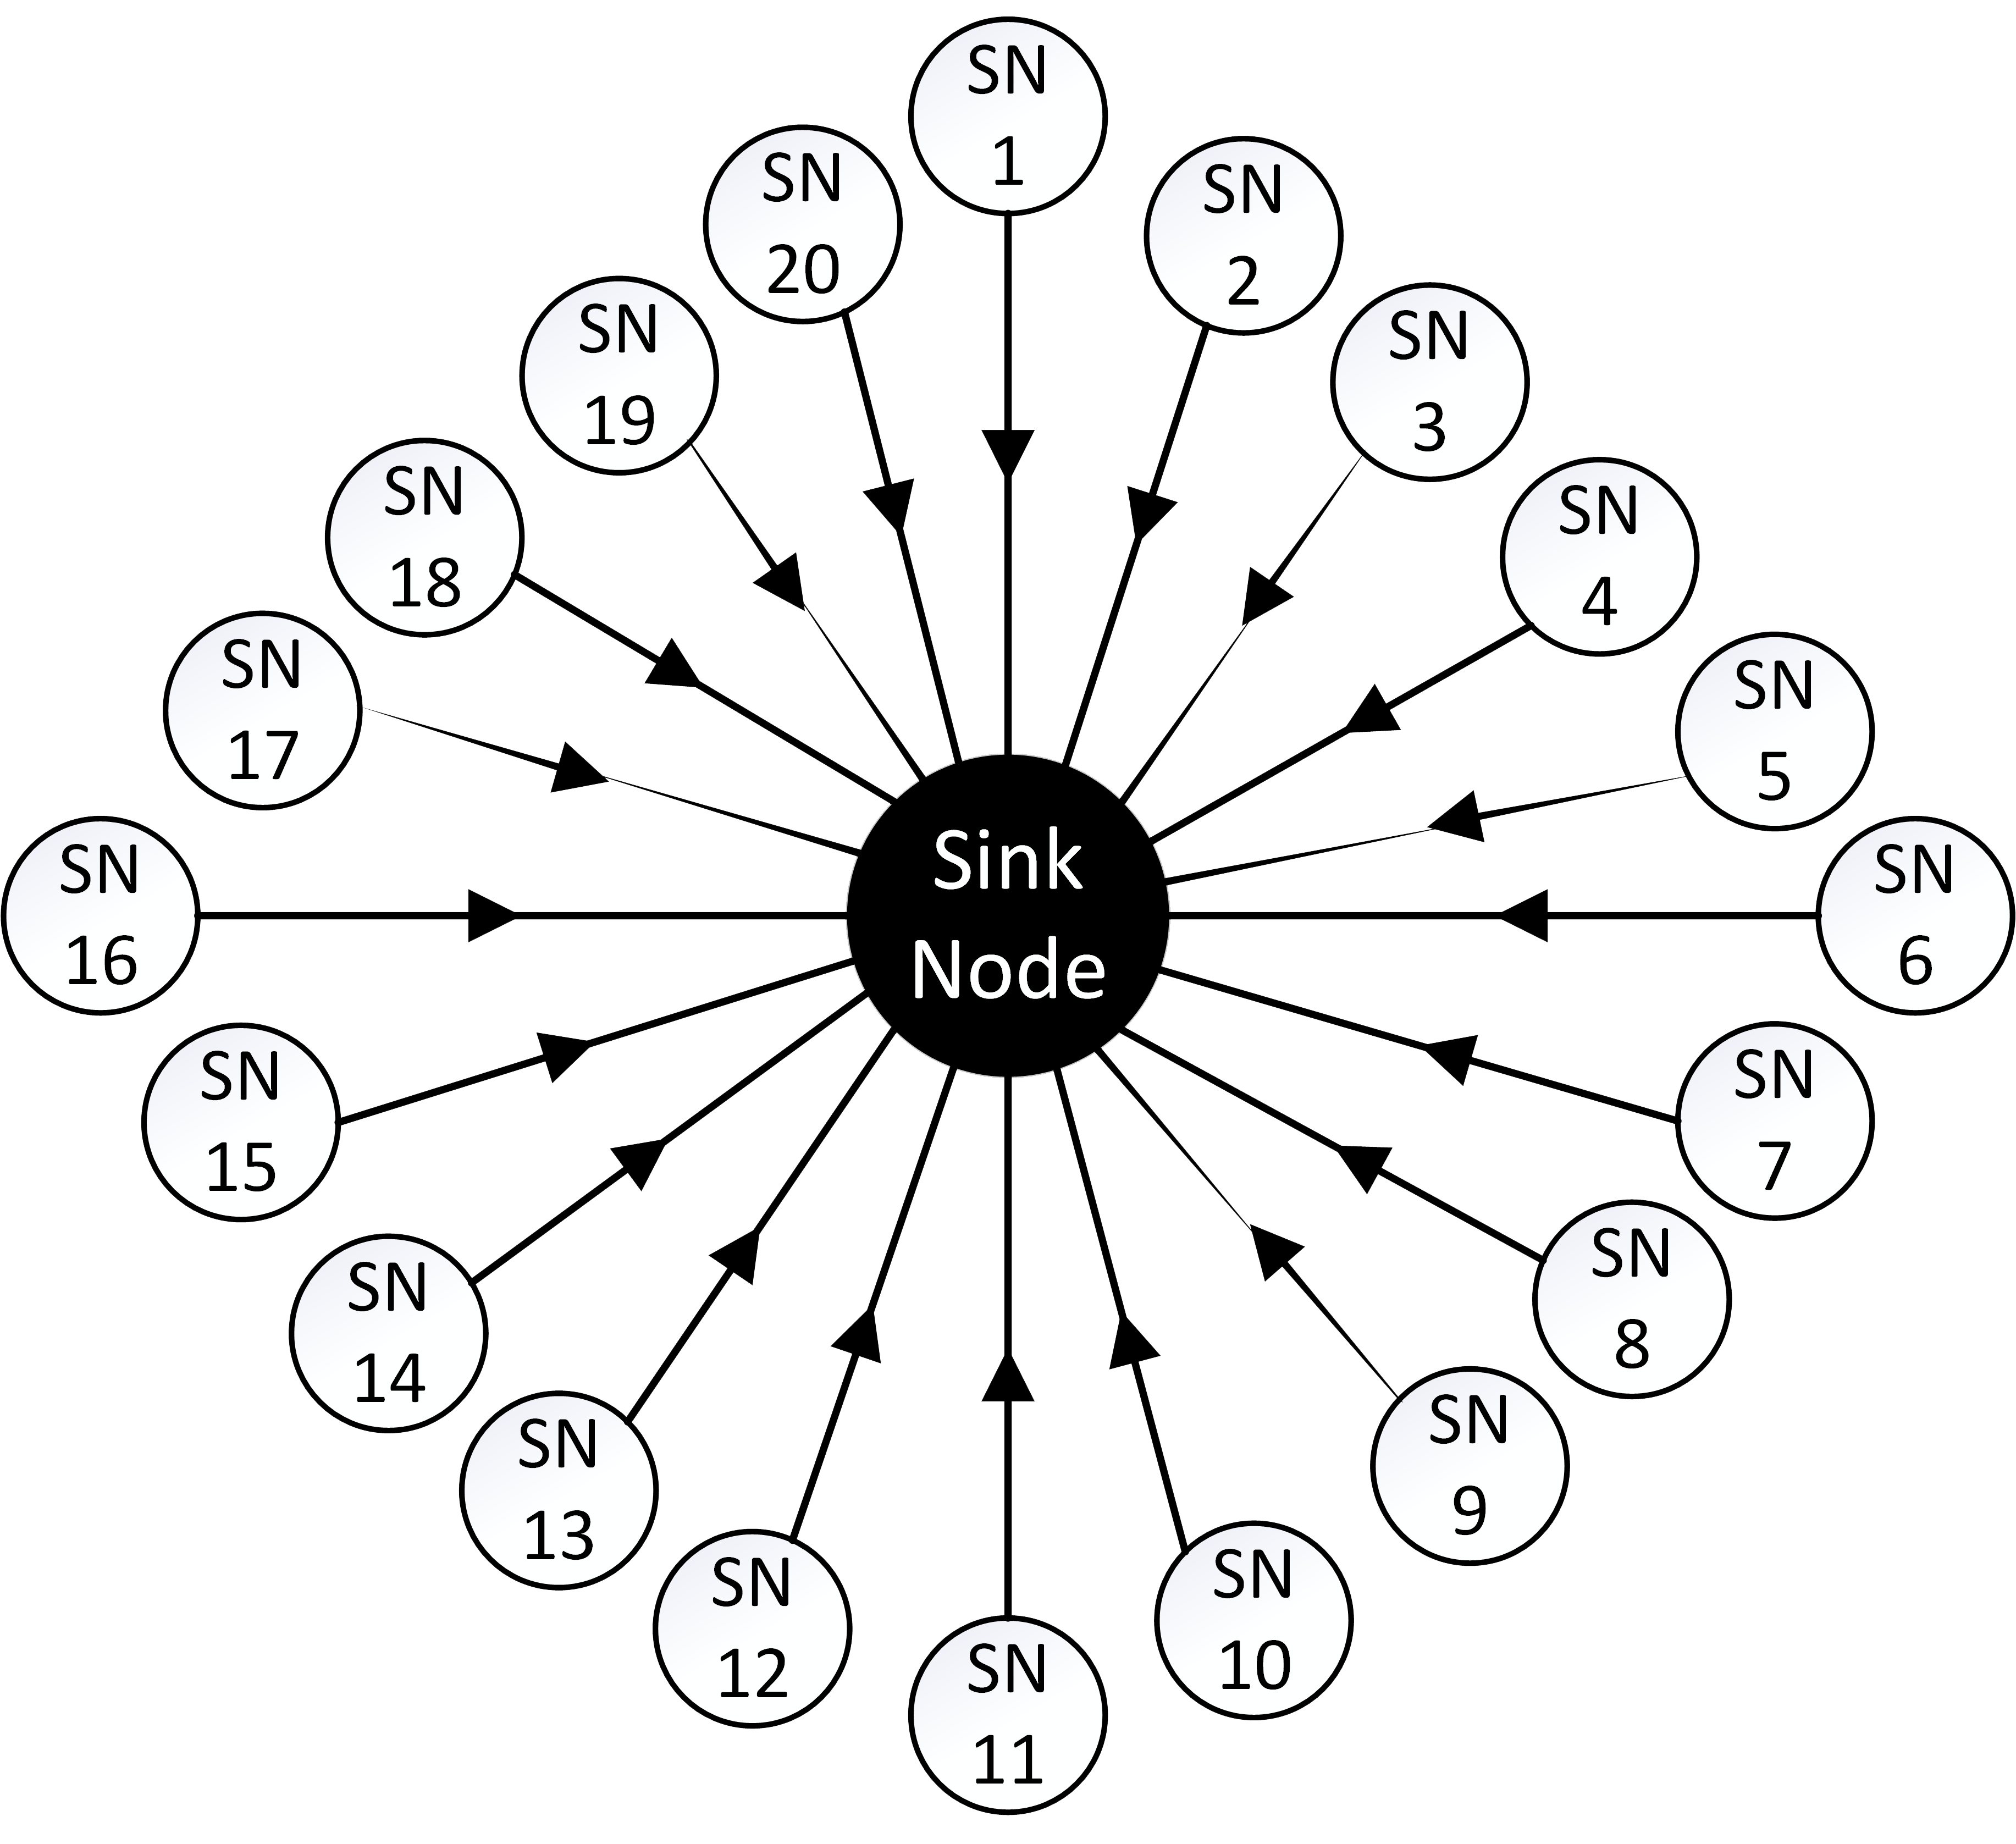
\includegraphics[width=1\linewidth]{pics/kodok}
		\caption{Star topology}
		\label{fig:kodok}
	\end{figure}
\end{center}


\newpage
\vspace*{1.5 cm}
\begin{figure}
	\centering
	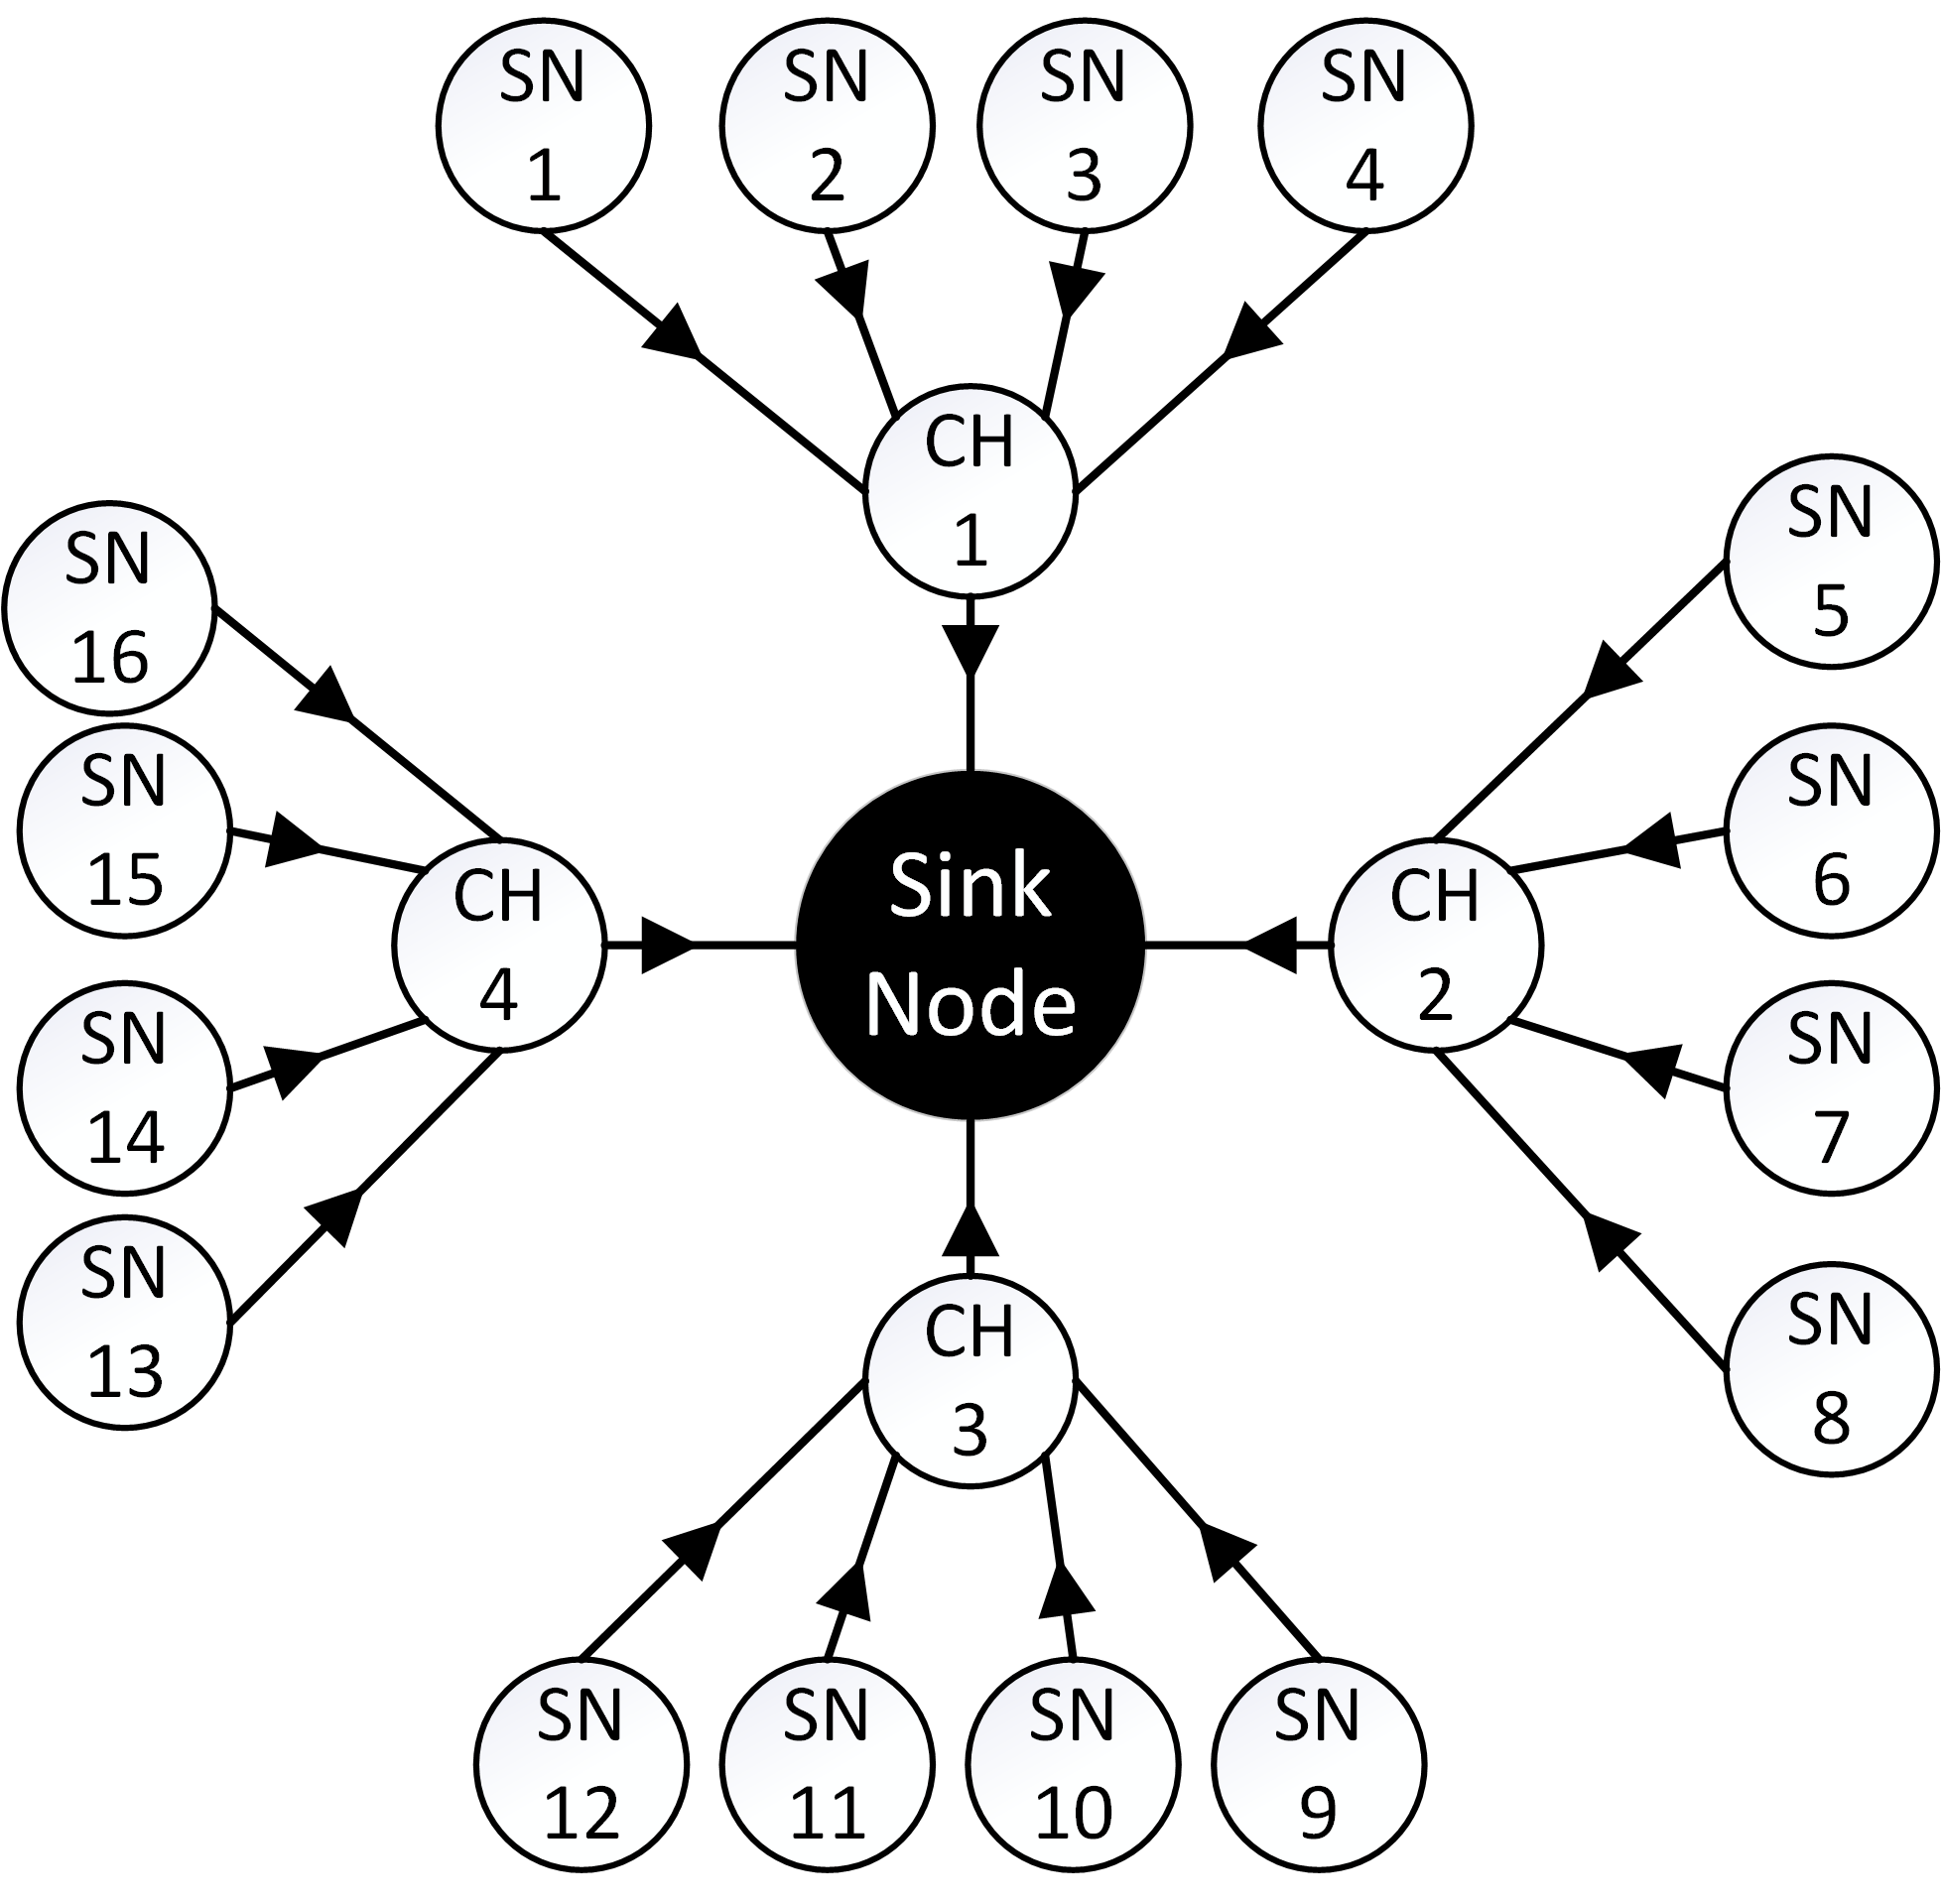
\includegraphics[width=1\linewidth]{pics/kuda}
	\caption{Cluster-based topology}
	\label{fig:kuda}
\end{figure}

\newpage
\vspace*{1.5 cm}
\begin{figure}
	\centering
	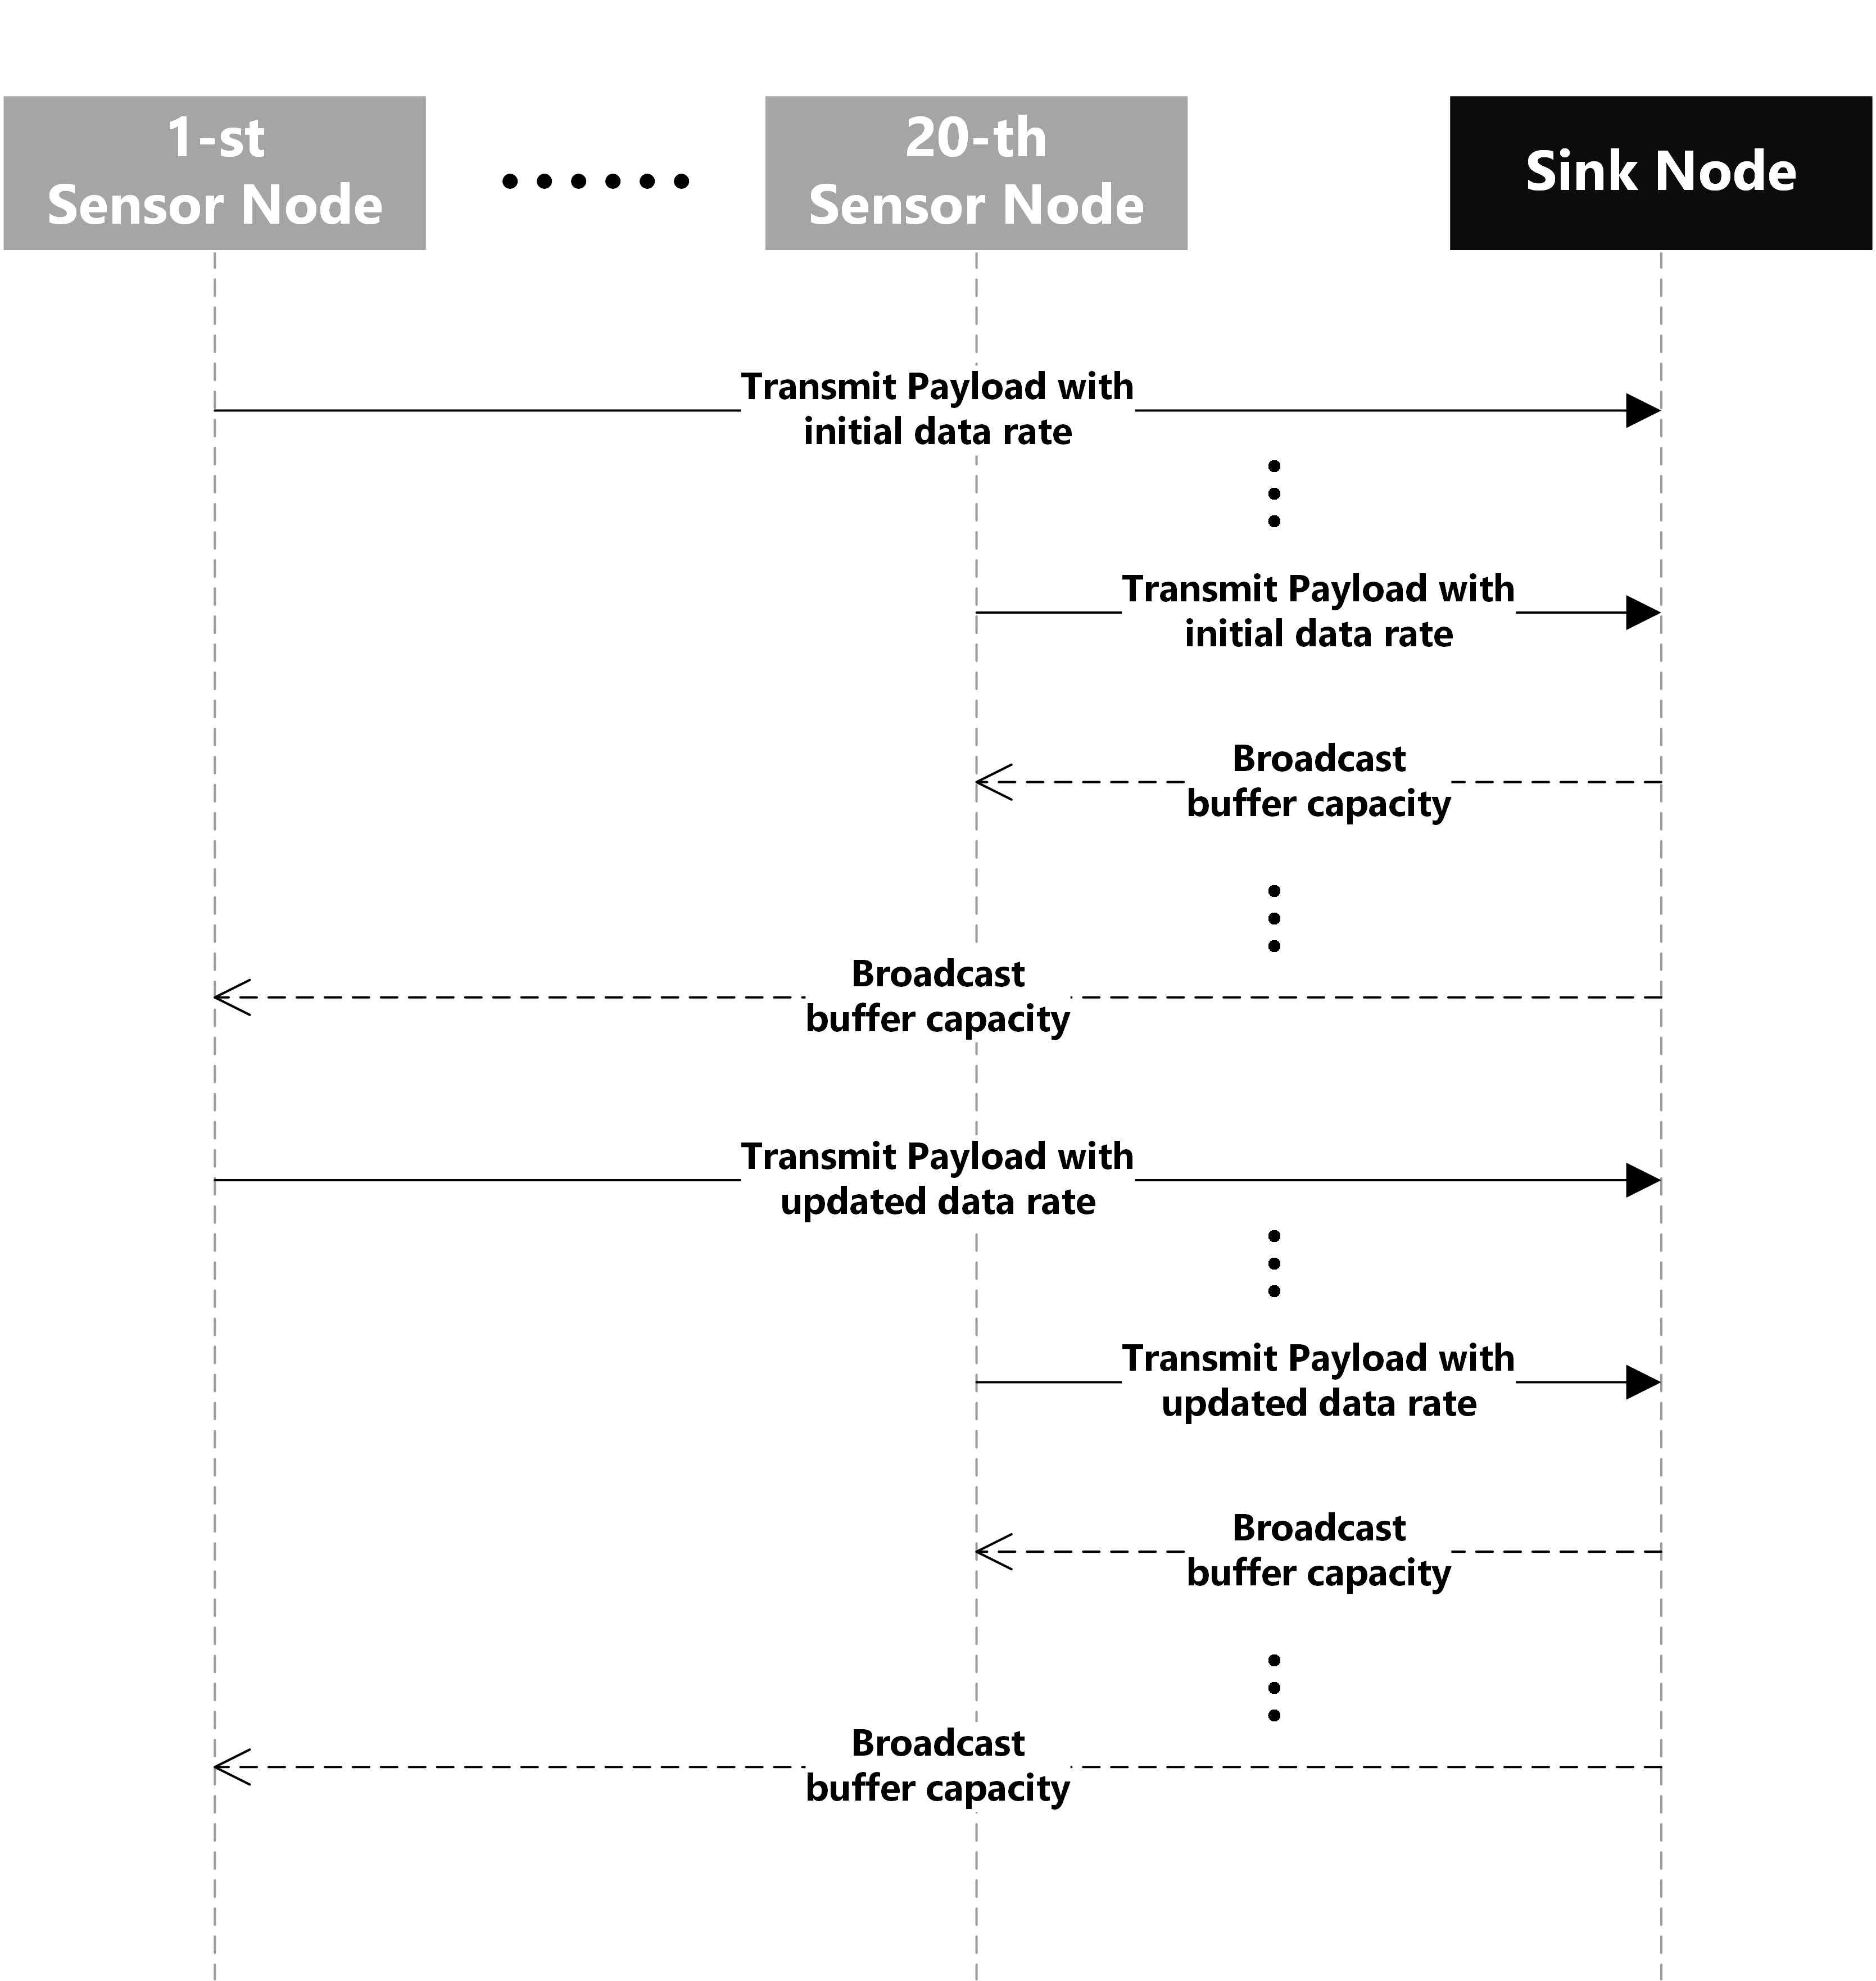
\includegraphics[width=1\linewidth]{pics/UntitledDiagram}
	\caption{Data flow of star topology}
	\label{fig:untitled-diagram}
\end{figure}



\begin{figure}
	\centering
	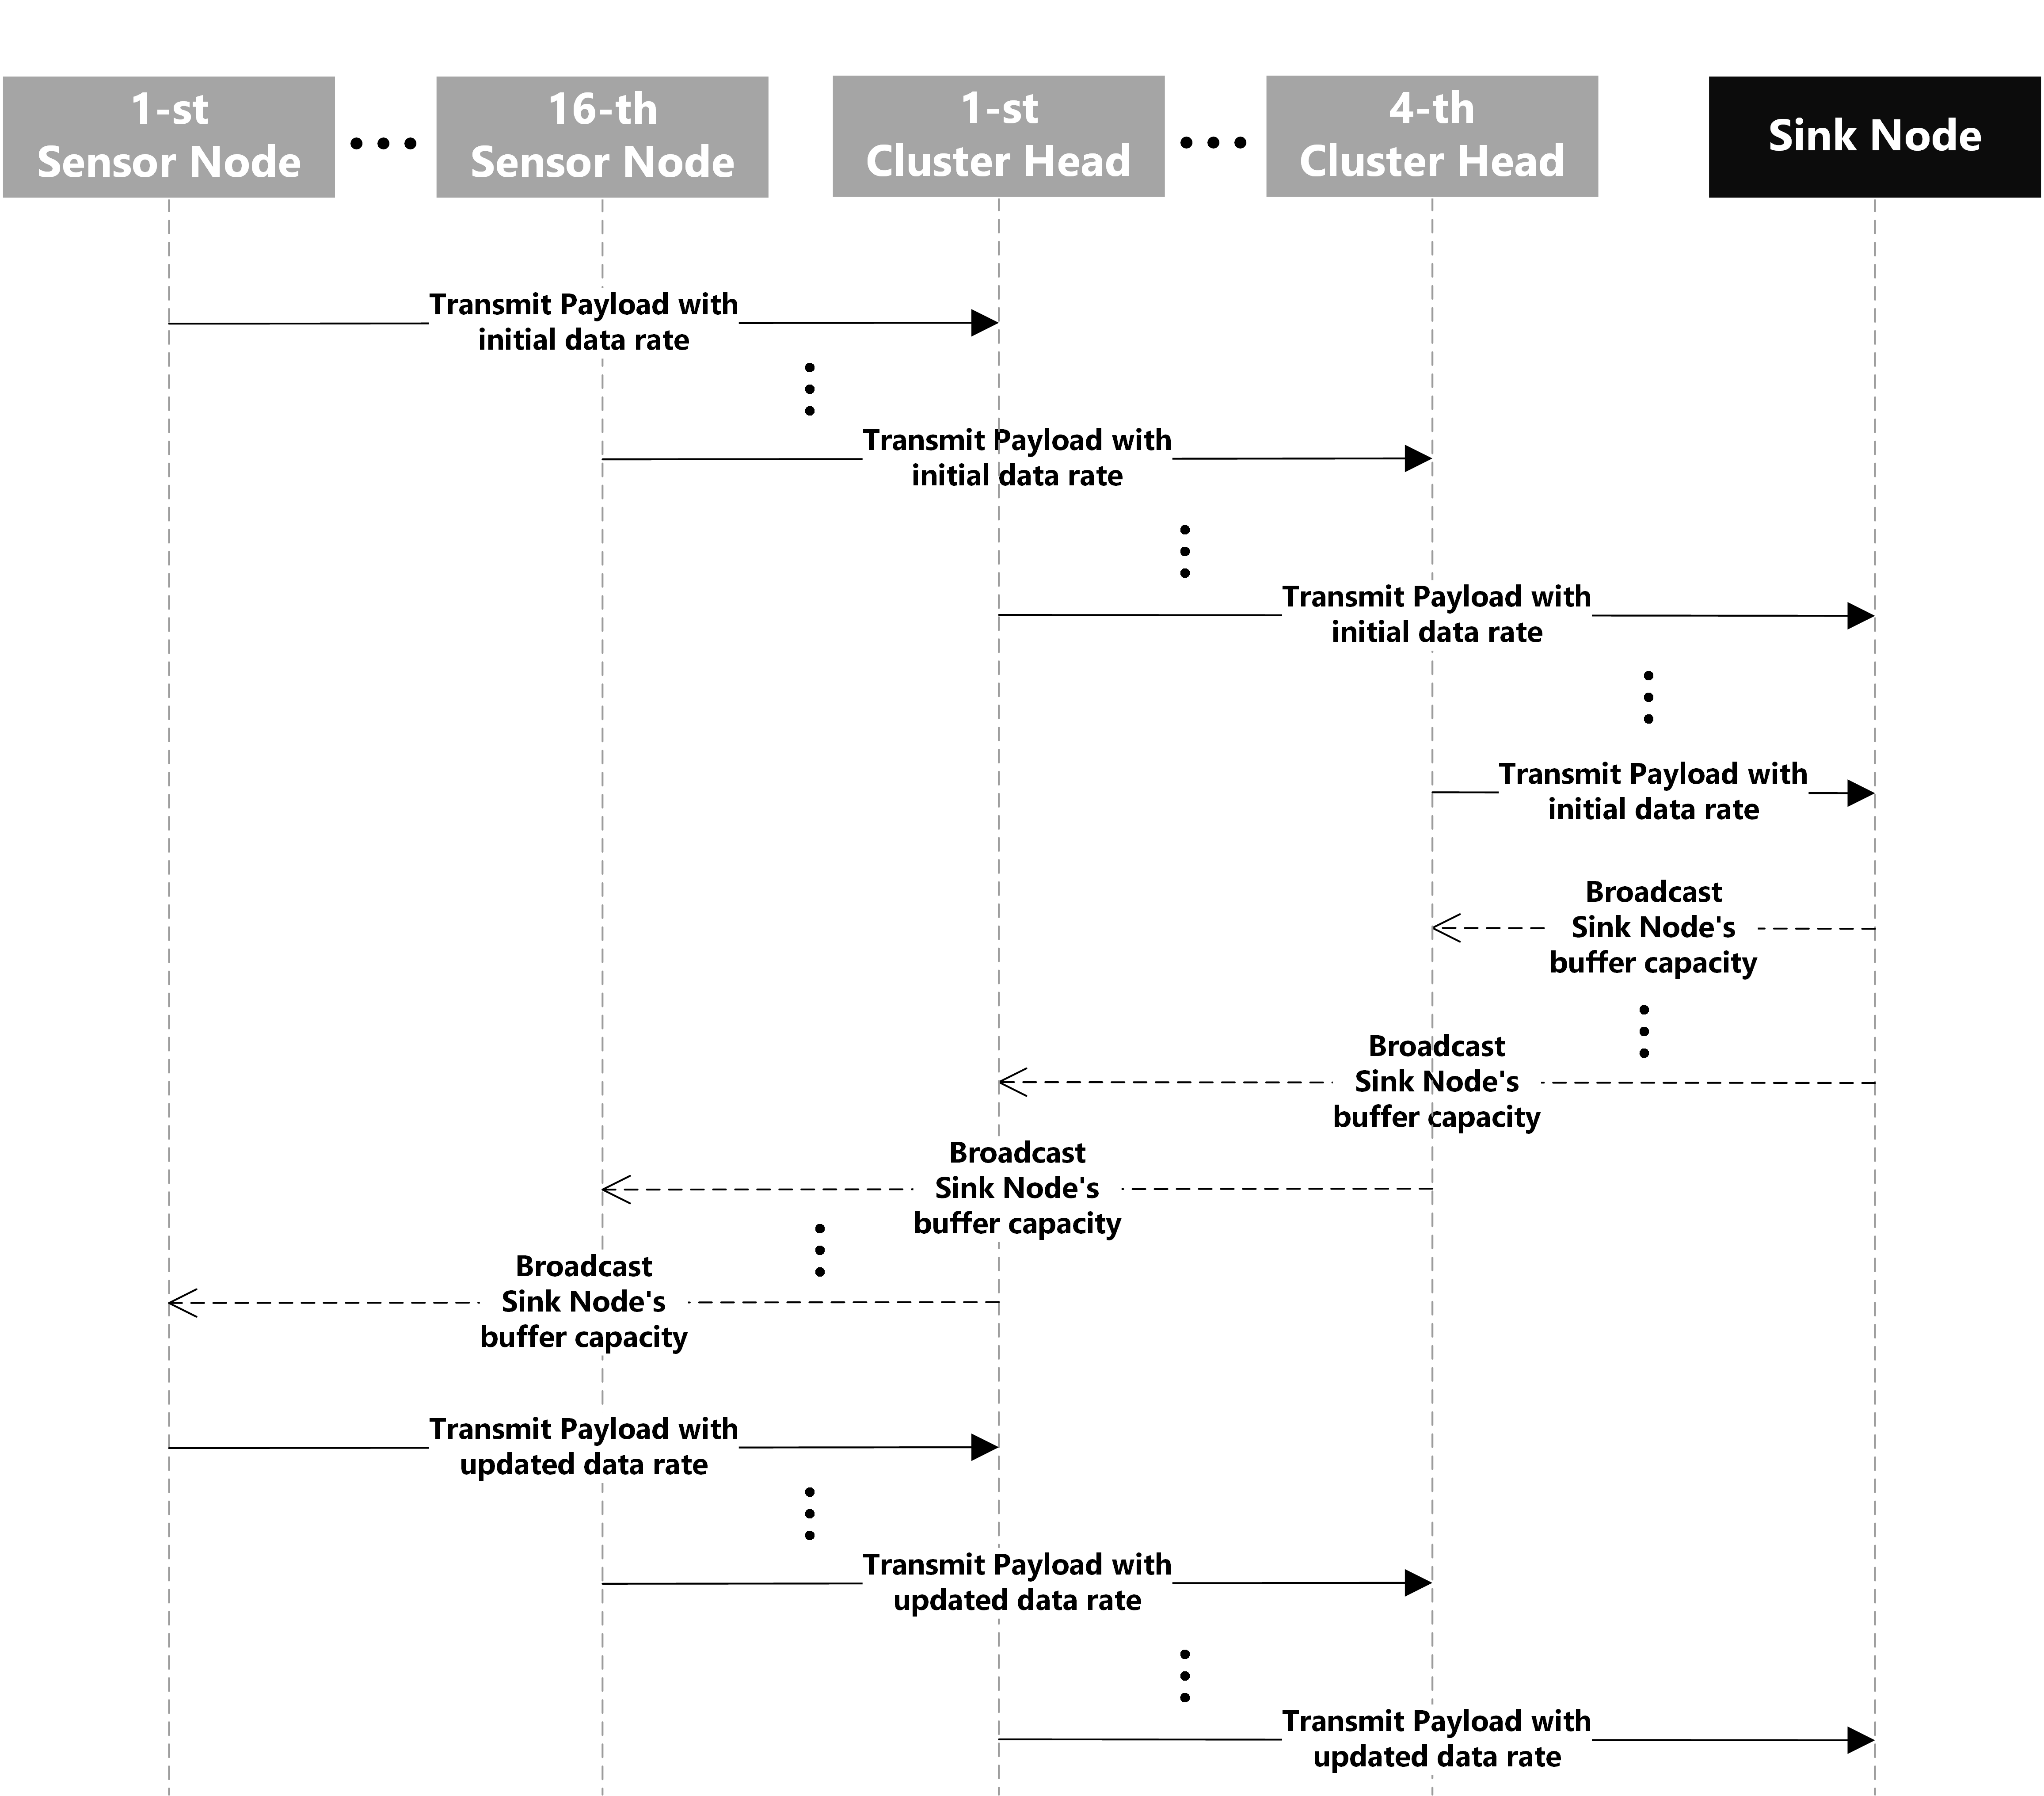
\includegraphics[width=1\linewidth]{pics/UntitledDiagram2}
	\caption{Data flow of mesh topology}
	\label{fig:untitled-diagram2}
\end{figure}


\section{Proposed DA for Congestion Control in IIoT}


The DA begins by generating a set of random solutions. In each iteration, the velocity and position of each dragonfly are updated using Eq. (\ref{eq1}) and Eq. (\ref{eq2}) alternatively, if they do not have neighboring solutions, Eq.
(\ref{dskimsegawon}) is used. The algorithm of DA is elaborated in Algorithm \ref{algo:1} with $MaxIteration$ as the maximum number of iteration.

\begin{algorithm}
	\caption{DA}
	\label{algo:1}
	\SetAlgoLined
	
	%\KwResult{Write here the result }
	Initialize $X_i$ and $V_i$ randomly\;
	\For {$t$ \textbf{to} $MaxIteration$}{
		\For {$i \leftarrow 1$ \textbf{to} $N$} {
			\eIf{$f(x_i) > X^-$}{
				$X^- \leftarrow f(x_i)$ \;
			}{}
			\eIf{$f(x_i) < X^+$}{
				$X^+ \leftarrow f(x_i)$ \;
			}{}
			Update $V$ with Eq.(\ref{eq1})\;
			\eIf{There is neighboring solutions}{Update $X$ with Eq.(\ref{eq2})\;}{Update $X$ with Eq.(\ref{dskimsegawon})\;}
			
		}
	}
\end{algorithm}

In this scheme, DA is used to optimize throughput and minimizing variance (to maintain fairness) by approaching $\alpha$ and $\beta$ as input with constraints as expressed in Inequality (\ref{ineq1}) and Inequality (\ref{ineq2}). The objective function $f(\alpha, \beta)$ is calculated in Algorithm~\ref{algo:2} with $M$ as the number of samples. The penalty method is used to give a penalty if the solution is beyond the constraints with the addition of a huge number. 

It must be noted that in DA, each agent should be bounded to minimize searching effort. The lower bound has been already determined by Inequality (\ref{ineq1}). Moreover, the upper bound is set to $10$ for simplicity.

\begin{algorithm}
	\caption{Objective Function}
	\label{algo:2}
	\SetAlgoLined
	\SetKwInOut{Input}{Input}\SetKwInOut{Output}{Output}
	\Input{$\alpha$ and $\beta$}
	\Output{$f(\alpha,\beta)$}
	\BlankLine
	$sum \leftarrow 0$\; 
	\For{$t \leftarrow 1$ \textbf{to} $M$}
	{
		$sum \leftarrow sum + \frac{1}{X(t)}$\; %$x(t)$ from Eq.(\ref{horse})
	}
	\eIf{$(\beta > \alpha)$ and ($\beta - \alpha \geq n \times (1- \alpha)$)}{
		$f(\alpha,\beta)= \frac{sum}{M} \times VAR(X(t))$\;
	}{
		$f(\alpha,\beta)= \infty $\;
		
	}
\end{algorithm}